\documentclass{discussion}

\usepackage{framed}
\usepackage[position=b]{subcaption}
\DeclareMathOperator{\Parents}{Parents}
\DeclareMathOperator{\NonDesc}{NonDesc}
\newcommand{\G}{\mathcal{G}}
\newcommand{\I}{\mathcal{I}}

\begin{document}

% Lecture Info
\lecture{7}{Probabilistic Graphical Models}{Benjamin R. Bray}

%\begin{exercise}
%\begin{example}

%%%% INTRODUCTION %%%%%%%%%%%%%%%%%%%%%%%%%%%%%%%%%%%%%%%%%%%%%%%%%%%%%%%%%%%%%%%%%%%%%%%%%%%%%%

This week in lecture, we introduced \textbf{Probabilistic Graphical Models}, which are a very elegant and powerful way to model the \textit{independence structure} of complex data.  So far, we have covered only simple probabilistic models like linear regression, logistic regression, and Naive Bayes.   Graphical models provide us with a language for expressing more complex probabilistic models.  Here are a few advantages of using graphical models:

\begin{itemize}
\item \textbf{Transparency.}  All modeling assumptions are explicitly encoded in the graph structure of a probabilistic model and the accompanying distributions. 
\item \textbf{Interpretability.} compared to i.e. neural networks or random forest models, whose learned parameters are hard to interpret.  In addition, because graphical models are \textit{probabilistic}, we can easily determine confidence intervals for our estimates, which matters when machine learning algorithms are used to make important real-world decisions (diagnosis, trading, self-driving cars, etc.).
\item \textbf{Modularity.}  Graphical models can be easily combined and modified, and it is easy to adapt old models to new applications.  Sometimes it's even useful to "nest" one graphical model inside another!
\end{itemize}

\begin{framed}
\textbf{Fair Warning:} We'll be using probability extensively in this section of the course, and it's important that you have a good grasp of the basics!  Conditional independence and Bayes' rule will be especially important.  Check Piazza for a list of concepts we expect you to know.
\end{framed}


%%%% CONDITIONAL INDEPENDENCE %%%%%%%%%%%%%%%%%%%%%%%%%%%%%%%%%%%%%%%%%%%%%%%%%%%%%%%%%%%%%%%%%%

Bayesian networks, which we define below, can be interpreted as a compact way of encoding conditional independence assumptions.  First, recall the concept of independence:

\begin{definition}
We say events or variables $X$ and $Y$ are \textbf{independent}, written $(X \perp Y)$, if
    \begin{equation*}
    P(X \mid Y) = P(X) \quad \text{or} \quad P(Y) = 0
    \end{equation*}
\end{definition}

While independence is a useful property, it is not often that we encounter two independent events in practice.  More commonly, two events are independent only if we have information about a third event.

\begin{definition}
We say events or variables $X$ and $Y$ are \textbf{conditionally independent} given $Z$, which we write as $(X \perp Y \mid Z)$, if
    \begin{equation*}
    P(X|Y,Z) = P(X|Z)
    \end{equation*}
\end{definition}

% Example:  Stanford/MIT
\begin{example} (Koller, \textit{Probabilistic Graphical Models})
For example, suppose we want to reason about the chance that a student is accepted to graduate studies at Stanford or MIT.  Denote by \textit{Stanford} the event "admitted to Stanford" and by \textit{MIT} the event "admitted to MIT."  In most reasonable distributions, these two events are not independent.  If we learn that a student was admitted to Stanford, then our estimate of her probability of bveing accepted at MIT is now higher, since it is a sign that she is a promising student.  

Now, suppose both universities base their decisions only on the student's grade point average, and we know that our student has a GPA of A.  In this case, we might argue that learning that the student was admitted to Stanford should not change the probability that she will be admitted to MIT:  her GPA already encodes all relevant information.  Formally, we have
    \begin{equation*}
    P(MIT \mid Stanford, GradeA) = P(MIT \mid GradeA)
    \end{equation*}
In this case, we say \textit{MIT} is conditionally independent of \textit{Stanford} given \textit{GradeA}.
\end{example}

\begin{exercise}
Let $X,Y,Z,W$ be events or random variables.  Show that conditional independence satisfies the following properties:
    \begin{itemize}
    \item \textbf{Symmetry:}  $(X \perp Y \mid Z) \implies (Y \perp X \mid Z)$
    \item \textbf{Decomposition:} $(X \perp Y,W \mid Z) \implies (X \perp Y \mid Z)$
    \item \textbf{Weak Union:} $(X \perp Y,W \mid Z) \implies (X \perp Y \mid Z,W)$
    \item \textbf{Contraction:} $(X \perp W \mid Z,Y) \wedge (X \perp Y \mid Z) \implies (X \perp Y,W \mid Z)$
    \end{itemize}
\end{exercise}

%%%% BAYESIAN NETWORKS %%%%%%%%%%%%%%%%%%%%%%%%%%%%%%%%%%%%%%%%%%%%%%%%%%%%%%%%%%%%%%%%%%%%%%%%%
\section{Bayesian Networks}

A Bayesian network is one type of graphical model that encodes a set of independence assumptions among a set of random variables with a graph.  At a high level, the structure of a Bayesian network tells us which relationships between variables we believe to be most important for solving the problem at hand.  Here is the formal definition of a Bayesian network from lecture:

\begin{definition}
A \textbf{Bayesian network} $\G$ is a directed acyclic graph whose nodes represent random variables $X_1, \dots, X_n$.  Let $\Parents(X_k)_\G$ denote the parents of $X_k$ in $\G$ and $\NonDesc(X_k)_\G$ denote the variables in the graph that are not descendants of $X_k$.  Then $\G$ encodes the following set of conditional independence assumptions, called the \textbf{local independencies}, and denoted by $\I_{\ell}(\G)$.
    \begin{equation*}
    \text{For each variable $X_k$}:  (X_k \perp \NonDesc_\G(X_k) \mid \Parents_\G(X_k))
    \end{equation*}
\end{definition}%

\noindent This definition looks scary and technical, but over the next few weeks we will work with many examples and working with these graphs will become second-nature.  For now, whenever you get confused, remember this one important fact:

\begin{framed} \centering
Every variable $X_k \in \G$ is conditionally independent of its nondescendants, given its parents.
\end{framed}

% Exercise:  Cycles
\begin{exercise}
Why must we require that the graphs be acyclic?  What happens if there are cycles?
\end{exercise}

% Exercise:  Parents & Nondescendants
\begin{exercise}
Identify the parents and nondescendants for each node in every graph in Figure \ref{fig:pgms}.
\end{exercise}

%% Naive Bayes --------------------------------------------------------------------------------
\subsection{Example: Naive Bayes}

Naive Bayes is the simplest nontrivial example of a graphical model.  The corresponding Bayesian network, shown in Figure \ref{fig:naive-bayes}, was briefly discussed in lecture, but let's go through it a little more carefully.

% Exercise:  Naive Bayes Local Independencies
\begin{exercise}
List all local independencies $\I_\G$ encoded by the graph in Figure \ref{fig:naive-bayes}.
\end{exercise}

\begin{example}
Show directly that the independence assumptions made by Bayesian network in Figure \ref{fig:naive-bayes} correspond exactly the Naive Bayes assumption.
\end{example}

\begin{figure*}[h!tb]
    \centering
    \begin{subfigure}[t]{0.33\textwidth}
        \centering
        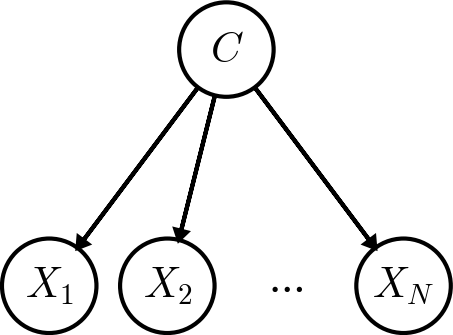
\includegraphics[height=1.2in]{images/naive-bayes}
        \caption{Naive Bayes \label{fig:naive-bayes}}
    \end{subfigure}%
    ~ 
    \begin{subfigure}[t]{0.33\textwidth}
        \centering
        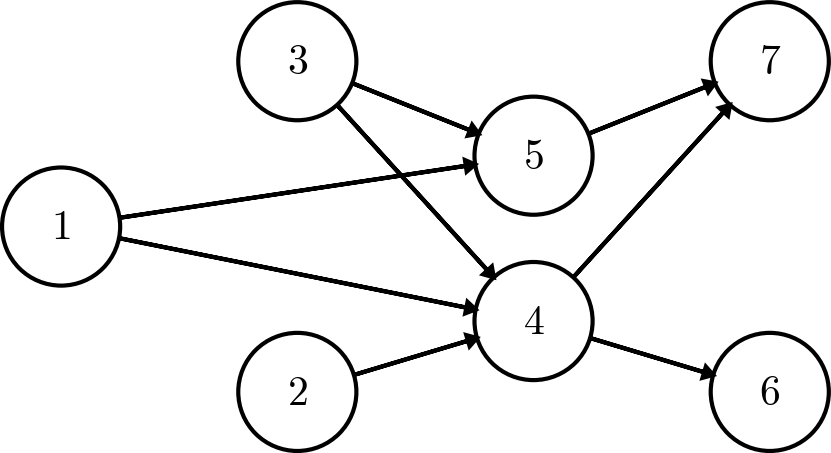
\includegraphics[height=1.2in]{images/topological}
        \caption{Topological Sort}
    \end{subfigure}%
    ~ 
    \begin{subfigure}[t]{0.33\textwidth}
        \centering
        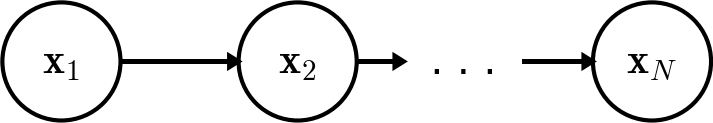
\includegraphics[height=0.3in]{images/markov-chain}
        \caption{Markov Chain \label{fig:markov-chain}}
    \end{subfigure}%
    \caption{\label{fig:pgms} Three simple Bayesian networks.}
\end{figure*}

%% Factorization Theorem ----------------------------------------------------------------------
\pagebreak
\section{From Networks to Factorizations}

\begin{theorem}[Factorization]
Suppose the network $\G$ is an I-map for $P$, that is, the distribution $P$ satisfies the independence assumptions contained in $\G$.  $X_1, \dots, X_n$ is any \textbf{topological sorting} of the nodes of $\G$, then $P$ \textbf{factorizes} according to $\G$ in the following way:
    \begin{equation*}
    P(X_1,\dots,X_n)
    = \prod_{k=1}^n P(X_k \mid \Parents_\G(X_k))
    \end{equation*}
\end{theorem}

\begin{proof}
Once we have topologically sorted nodes $X_1, \dots, X_n$, the chain rule for probability yields
    \begin{equation*}
    P(X_1,\dots,X_n)
    = P(X_1) P(X_2 \mid X_1) \cdots P(X_n | X_1, \dots, X_{n-1})
    = \prod_{k=1}^n P(X_k \mid X_1, \dots, X_{k-1})
    \end{equation*}
The nodes are topologically sorted, so all parents of $X_k$ are in the range $X_1, \dots, X_{k-1}$, and the rest of these nodes must be nondescendants.  Because $X_k$ is conditionally independent of its nondescendants given its parents, we can delete the nondescendants frmo this list when conditioning.  Therefore, $P(X_k \mid X_1, \dots, X_{k-1}) = P(X_k \mid \Parents_\G(X_k))$.  For a more rigorous proof, see the lecture notes.
\end{proof}

% Example:  Naive Bayes
\begin{example}
After establishing the factorization theorem, it is clear that Figure \ref{fig:naive-bayes} is indeed Naive Bayes.
\end{example}

The factorization theorem is incredibly useful for building \textbf{generative models}, which describe our assumptions about how the observed data is generated.  Using the factorization theorem, we can interpret any Bayesian network as a generative model.

%% Example:  Markov Chains -------------------------------------------------------------------
\subsection{Example:  Markov Chains}

A \textbf{Markov chain} is a simple probabilistic model used for describing sequences, usually discretized in either time or space.  The corresponding graphical model is shown in Figure \ref{fig:markov-chain}.  Markov chains are often called \textit{local} or \textit{memoryless} models because if the value at position $k$ in the chain is known, then past values do not influence our predictions of future values.  While not entirely true in general, this assumption can simplify inference in complex settings like weather forecasing, finance, and natural language processing.  Usually, we assume all variables in a Markov chain have the same type.

\begin{exercise}
List all local independence assumptions made by the Markov Chain model in Figure \ref{fig:markov-chain}.
\end{exercise}

\begin{exercise}
By the factorization theorem, the joint distribution for a Markov chain factorizes as
    \begin{equation*}
    P(X_1,\dots,X_n)
    = \prod_{k=1}^n P(X_k \mid \Parents_\G(X_k))
    = \prod_{k=1}^n P(X_k \mid X_{k-1})
    \end{equation*}
Using this factorization, interpret Markov Chains as a generative model.  It may help to think of the random variables $X_1, \dots, X_n$ as words in a sentence, a robot's position at time $t$, or the weather forecast $\{ Rainy, Sunny \}$ on day $d$.  Draw a transition diagram for the model.
\end{exercise}

%% From Factorizations to Networks -----------------------------------------------------------
\section{From Factorizations to Networks}

If we know the independence structure of a joint distrubution over some variables, we can write down a corresponding Bayesian network that encodes these independencies.  Remember that there are multiple valid answers!  The complete graph on $n$ nodes is a valid Bayesian network for any variables $X_1, \dots, X_n$.

\begin{exercise}
Draw a Bayesian network for each factored joint distribution below.
    \begin{itemize}
    \item $P(A,B,C,D)$
    \item $P(A,B,C) = P(A)P(B|A)P(C|B)$
    \item $P(A,B,C,D,E) = P(A)P(B)P(C|A,B)P(D)P(E|C,D)$
    \end{itemize}
\end{exercise}

We can also be more concrete!  Suppose we are given a generative model, complete with distributions that tell us how to generate data.  We can use this information to come up with a Bayesian network that fits the independence assumptions of the generative model.

\begin{example}
TODO
\end{example}

\end{document}
